\documentclass[exercice]{thedocument}%
\usepackage{tkz-euclide}%
\startdatakeys
\source{}
\cycle{}
\competencesDuSocle{}
\connaissancesRequises{}
\competencesTravaillees{}
\enddatakeys
\begin{document}%
\begin{minipage}[t]{.5\linewidth}
    Alexis a décrit la figure ci-contre, mais sa feuille est déchirée. Voici
    une partie du début de son texte.\par
    {\centering\pdf{6eme_Transmath_186_28_1}\par}
    Recopier ces lignes, les compléter et écrire la suite.%
    \answerspace{2.5cm}
\end{minipage}\hskip20pt
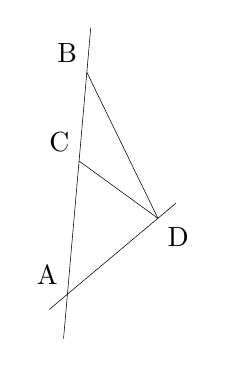
\begin{tikzpicture}[scale=0.5,rotate=40, baseline=(current bounding box.north)]
    \coordinate[label=above left:A](A)at(0,0);
    \coordinate[label=above left:B](B)at(4,4);
    \path(A)--(B)coordinate[pos=0.6,label=above left:C](C);
    \coordinate[label=below right:D](D)at(3,0);
    \tkzDrawLines(A,B A,D)
    \tkzDrawSegments(C,D B,D)
\end{tikzpicture}
\end{document}
